\pdfminorversion=4 % for acroread
%\documentclass[aspectratio=169,t,xcolor={usenames,dvipsnames}]{beamer}
\documentclass[aspectratio=169,t,handout,xcolor={usenames,dvipsnames}]{beamer}
\usepackage{../beamerstyle}
\usepackage{dsfont}
\usepackage{bm}
\usepackage[english]{babel}
\usepackage[utf8]{inputenc}
\usepackage{graphicx}
\usepackage{algorithm}
\usepackage[ruled,vlined,algo2e,linesnumbered]{algorithm2e}
%\usepackage[boxed,vlined]{algorithm2e}
\usepackage{hyperref}
\usepackage{booktabs}
\usepackage{mathtools}

\usepackage{amsmath,amssymb}
\usepackage{listings}
\lstset{frame=lines,framesep=3pt,numbers=left,numberblanklines=false,basicstyle=\ttfamily\small}

\usepackage{subfig}
\usepackage{multicol}
%\usepackage{appendixnumberbeamer}
%
\usepackage{tcolorbox}

\usepackage{pgfplots}
\usepackage{tikz}
\usetikzlibrary{trees} 
\usetikzlibrary{shapes.geometric}
\usetikzlibrary{positioning,shapes,shadows,arrows,calc,mindmap}
\usetikzlibrary{positioning,fadings,through}
\usetikzlibrary{decorations.pathreplacing}
\usetikzlibrary{intersections}
\usetikzlibrary{positioning,fit,calc,shadows,backgrounds}
\pgfdeclarelayer{background}
\pgfdeclarelayer{foreground}
\pgfsetlayers{background,main,foreground}
\tikzstyle{activity}=[rectangle, draw=black, rounded corners, text centered, text width=8em]
\tikzstyle{data}=[rectangle, draw=black, text centered, text width=8em]
\tikzstyle{myarrow}=[->, thick, draw=black]

% Define the layers to draw the diagram
\pgfdeclarelayer{background}
\pgfdeclarelayer{foreground}
\pgfsetlayers{background,main,foreground}

%\usepackage{listings}
%\lstset{numbers=left,
%  showstringspaces=false,
%  frame={tb},
%  captionpos=b,
%  lineskip=0pt,
%  basicstyle=\ttfamily,
%%  extendedchars=true,
%  stepnumber=1,
%  numberstyle=\small,
%  xleftmargin=1em,
%  breaklines
%}

 
\definecolor{blue}{RGB}{0, 74, 153}

\usetheme{Boadilla}
%\useinnertheme{rectangles}
\usecolortheme{whale}
\setbeamercolor{alerted text}{fg=blue}
\useoutertheme{infolines}
\setbeamertemplate{navigation symbols}{\vspace{-5pt}} % to lower the logo
\setbeamercolor{date in head/foot}{bg=white} % blue
\setbeamercolor{date in head/foot}{fg=white}
\setbeamercolor{author  in head/foot}{bg=white} %blue
\setbeamercolor{title in head/foot}{bg=white} % blue
\setbeamercolor{title}{fg=white, bg=blue}
\setbeamercolor{block title}{fg=white,bg=blue}
\setbeamercolor{block body}{bg=blue!10}
\setbeamercolor{frametitle}{fg=white, bg=blue}
\setbeamercovered{invisible}

\makeatletter
\setbeamertemplate{footline}
{
  \leavevmode%
  \hbox{%
  \begin{beamercolorbox}[wd=.333333\paperwidth,ht=2.25ex,dp=1ex,center]{author in head/foot}%
%    \usebeamerfont{author in head/foot}\insertshortauthor
  \end{beamercolorbox}%
  \begin{beamercolorbox}[wd=.333333\paperwidth,ht=2.25ex,dp=1ex,center]{title in head/foot}%
    \usebeamerfont{title in head/foot}\insertshorttitle
  \end{beamercolorbox}%
  \begin{beamercolorbox}[wd=.333333\paperwidth,ht=2.25ex,dp=1ex,right]{date in head/foot}%
    \usebeamerfont{date in head/foot}\insertshortdate{}\hspace*{2em}
%    \insertframenumber\hspace*{2ex} 
  \end{beamercolorbox}}%
  \vskip0pt%
}
\makeatother

%\pgfdeclareimage[height=1.2cm]{automl}{images/logos/automl.png}
%\pgfdeclareimage[height=1.2cm]{freiburg}{images/logos/freiburg}

%\logo{\pgfuseimage{freiburg}}

\renewcommand{\comment}[1]{
	\noindent
	%\vspace{0.25cm}
	{\color{red}{\textbf{TODO:} #1}}
	%\vspace{0.25cm}
}
\newcommand{\notefh}[1]{\textcolor{red}{\textbf{FH:} #1}}
\renewcommand{\comment}[1]{}
\newcommand{\hide}[1]{}
\newcommand{\cemph}[2]{\emph{\textcolor{#1}{#2}}}

\newcommand{\lit}[1]{{\footnotesize\color{black!60}[#1]}}

\newcommand{\litw}[1]{{\footnotesize\color{blue!20}[#1]}}


\newcommand{\myframe}[2]{\begin{frame}[c]{#1}#2\end{frame}}
\newcommand{\myframetop}[2]{\begin{frame}{#1}#2\end{frame}}
\newcommand{\myit}[1]{\begin{itemize}#1\end{itemize}}
\newcommand{\myblock}[2]{\begin{block}{#1}#2\end{block}}


\newcommand{\votepurple}[1]{\textcolor{Purple}{$\bigstar$}}
\newcommand{\voteyellow}[1]{\textcolor{Goldenrod}{$\bigstar$}}
\newcommand{\voteblue}[1]{\textcolor{RoyalBlue}{$\bigstar$}}
\newcommand{\votepink}[1]{\textcolor{Pink}{$\bigstar$}}

\newcommand{\diff}{\mathop{}\!\mathrm{d}}
\newcommand{\refstyle}[1]{{\small{\textcolor{gray}{#1}}}}
\newcommand{\hands}[0]{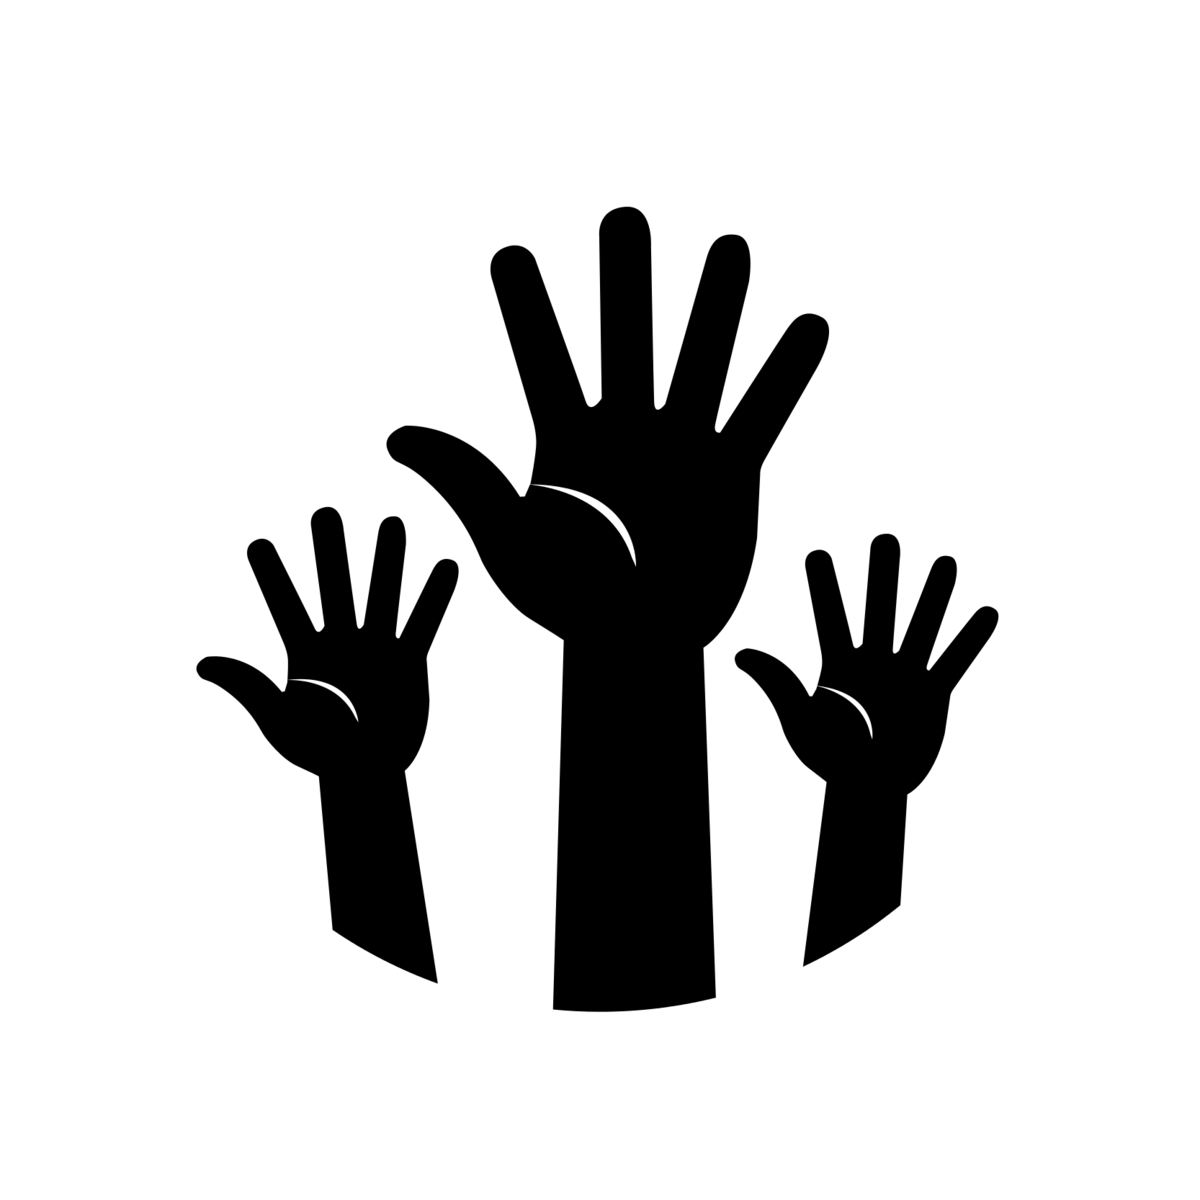
\includegraphics[height=1.5em]{images/hands}}
\newcommand{\transpose}[0]{{\textrm{\tiny{\sf{T}}}}}
\newcommand{\norm}{{\mathcal{N}}}
\newcommand{\cutoff}[0]{\kappa}
\newcommand{\instD}[0]{\dataset}
\newcommand{\insts}[0]{\mathcal{I}}
\newcommand{\inst}[0]{i}
\newcommand{\instI}[1]{i^{(#1)}}

% Iteration specific instance of variable/function/anything
% Introduced in the BO section, but moved up here to make it available within other macros
\newcommand{\iter}[2][\bocount]{{#2}^{(#1)}}

%--------HPO parameter macros-----------

% Parameter Configuration Space
\newcommand{\pcs}[0]{\pmb{\Lambda}}

% ???
\newcommand{\bx}[0]{\conf}

% Parameter Configuration
\newcommand{\conf}[0]{\pmb{\lambda}}

% Final Configuration
\newcommand{\finconf}[0]{\pmb{\hat{\lambda}}}

% Configuration corresponding to a given iteration -- better use \iter!
\newcommand{\confI}[1]{{\conf}^{(#1)}}

% Default Configuration
\newcommand{\defconf}[0]{{\conf}_{\text{def}}}

% Incumbent Configuration
\newcommand{\incumbent}[1][\bocount]{\iter[#1]{\finconf}}

% Optimal Configuration
\newcommand{\optconf}[0]{{\conf}^*}

% Configuration Space
\newcommand{\confs}[0]{\pcs}

%----------------------------------------

%\newcommand{\vlambda}[0]{\bm{\lambda}}
%\newcommand{\vLambda}[0]{\bm{\Lambda}}
\newcommand{\dataset}[0]{\mathcal{D}}
\newcommand{\datasets}[0]{\mathbf{D}}
\newcommand{\loss}[0]{L}
\newcommand{\risk}{\mathcal{R}}
\newcommand{\riske}{\mathcal{R}_{\text{emp}}}
\newcommand{\cost}[0]{c}
\newcommand{\costI}[1]{c^{(#1)}}

% Gaussian Process
\newcommand{\gp}{\mathcal{G}}
% Family of Objective Functions
\newcommand{\objF}{F}

%---------------BO Macros------------------

% BO loop counter
\newcommand{\bocount}{t}
% BO loop counter max, the counter runs from 1 to this value
\newcommand{\bobudget}{T}
% BO loop observation
\newcommand{\obs}[1][\conf]{\cost({#1})}
% BO loop observation space
\newcommand{\obsspace}{\mathcal{Y}}
% BO loop next observation
\newcommand{\bonextobs}{\obs[\iter{\conf}]}
% Acquisition Function, no args
\newcommand{\acq}{u}
% Standard Normal PDF
\newcommand{\pdf}{\phi}
% Standard Normal CDF
\newcommand{\cdf}{\Phi}
% Mean
\newcommand{\mean}{\mu}
% Standard Deviation
\newcommand{\stddev}{\sigma}
% Variance
\newcommand{\variance}{\sigma^2}
% Noise
\newcommand{\noise}{\nu}
% BO loop next selected sample
\newcommand{\bonextsample}{\confI{\bocount}}

% Single hyperparameter
\newcommand{\hyperparam}{\lambda}

% Single hyperparameter within a hyperparameter configuration
\newcommand{\hyperparami}[1][i]{{\hyperparam}_#1}

% Full definition of final configuration
\newcommand{\finconffull}{\incumbent[\bobudget]}

% Dataset
\newcommand{\datasetHPO}{{\dataset}_{HPO}}

% Dataset definition
\newcommand{\datasetHPOdef}{{\langle \bonextsample,\,\bonextobs \rangle}_{\bocount=1}^{\bobudget}}

% Double Display Fraction, forces large displays for everything in numerator and denominator
\newcommand\ddfrac[2]{\frac{\displaystyle #1}{\displaystyle #2}}

% Conditional Probability "Given That" Relation, source:https://tex.stackexchange.com/a/141685/205886
\newcommand\given[1][]{\:#1\vert\:}

% Expectation as a math operator
\DeclareMathOperator*{\E}{\mathbb{E}}

% Citation 
\newcommand{\source}[1]{
    \begin{flushright}
    	Source: \lit{#1}
    \end{flushright}
}
%-------------------------------------------

%Real numbers set
\newcommand{\realnum}{\mathbb{R}}
%Configuration space - do not use
%\newcommand{\configspace}{\Theta}
%Instances - do not use
%\newcommand{\instances}{\mathcal{I}}
%Expected value
\newcommand{\expectation}{\mathbb{E}}
%Kernel
\newcommand{\kernel}{\kappa}
%Constraint function
\newcommand{\constraintf}{c}
%Normal distribution
\newcommand{\normaldist}{\mathcal{N}}

% \renewcommand{\vec}[1]{\mathbf{#1}}
\newcommand{\hist}[0]{\dataset_{\text{Hist}}}
\newcommand{\param}[0]{p}
\newcommand{\algo}[0]{\mathcal{A}}
\newcommand{\algos}[0]{\mathbf{A}}
%\newcommand{\nn}[0]{N}
\newcommand{\feats}[0]{\mathcal{X}_{\text{meta}}}
\newcommand{\feat}[0]{\x_{\text{meta}}}
%\newcommand{\cluster}[0]{\vec{h}}
%\newcommand{\clusters}[0]{\vec{H}}
\newcommand{\perf}[0]{\mathbb{R}}
%\newcommand{\surro}[0]{\mathcal{S}}
\newcommand{\surro}[0]{\hat{\cost}}
\newcommand{\func}[0]{f}
\newcommand{\epm}[0]{\surro}
\newcommand{\portfolio}[0]{\mathbf{P}}
\newcommand{\schedule}[0]{\mathcal{S}}

% Machine Learning
\newcommand{\mdata}[0]{\dataset_{\text{meta}}}
\newcommand{\datasettrain}[0]{\dataset_{\text{train}}}
\newcommand{\datasetval}[0]{\dataset_{\text{val}}}
\newcommand{\datasettest}[0]{\dataset_{\text{test}}}
\newcommand{\x}[0]{\mathbf{x}}
\newcommand{\y}[0]{y}
\newcommand{\xI}[1]{\mathbf{x}^{(#1)}}
\newcommand{\yI}[1]{y^{(#1)}}
\newcommand{\fx}{f(\mathbf{x})}  % f(x), continuous prediction function
\newcommand{\Hspace}{\mathcal{H}} % hypothesis space where f is from
\newcommand{\fh}{\hat{f}}       % f hat, estimated prediction function

% Deep Learning
\newcommand{\weights}[0]{\theta}
\newcommand{\metaweights}[0]{\phi}


% reinforcement learning
\newcommand{\policies}[0]{\mathbf{\Pi}}
\newcommand{\policy}[0]{\pi}
\newcommand{\actionRL}[0]{a}
\newcommand{\stateRL}[0]{s}
\newcommand{\statesRL}[0]{\mathcal{S}}
\newcommand{\rewardRL}[0]{r}
\newcommand{\rewardfuncRL}[0]{\mathcal{R}}

\RestyleAlgo{algoruled}
\DontPrintSemicolon
\LinesNumbered
\SetAlgoVlined
\SetFuncSty{textsc}

\SetKwInOut{Input}{Input}
\SetKwInOut{Output}{Output}
\SetKw{Return}{return}

%\newcommand{\changed}[1]{{\color{red}#1}}

%\newcommand{\citeN}[1]{\citeauthor{#1}~(\citeyear{#1})}

\renewcommand{\vec}[1]{\mathbf{#1}}
\DeclareMathOperator*{\argmin}{arg\,min}
\DeclareMathOperator*{\argmax}{arg\,max}

%\newcommand{\aqme}{\textit{AQME}}
%\newcommand{\aslib}{\textit{ASlib}}
%\newcommand{\llama}{\textit{LLAMA}}
%\newcommand{\satzilla}{\textit{SATzilla}}
%\newcommand{\satzillaY}[1]{\textit{SATzilla'{#1}}}
%\newcommand{\snnap}{\textit{SNNAP}}
%\newcommand{\claspfolioTwo}{\textit{claspfolio~2}}
%\newcommand{\flexfolio}{\textit{FlexFolio}}
%\newcommand{\claspfolioOne}{\textit{claspfolio~1}}
%\newcommand{\isac}{\textit{ISAC}}
%\newcommand{\eisac}{\textit{EISAC}}
%\newcommand{\sss}{\textit{3S}}
%\newcommand{\sunny}{\textit{Sunny}}
%\newcommand{\ssspar}{\textit{3Spar}}
%\newcommand{\cshc}{\textit{CSHC}}
%\newcommand{\cshcpar}{\textit{CSHCpar}}
%\newcommand{\measp}{\textit{ME-ASP}}
%\newcommand{\aspeed}{\textit{aspeed}}
%\newcommand{\autofolio}{\textit{AutoFolio}}
%\newcommand{\cedalion}{\textit{Cedalion}}
\newcommand{\fanova}{\textit{fANOVA}}
\newcommand{\sbs}{\textit{SB}}
\newcommand{\oracle}{\textit{VBS}}

% like approaches
\newcommand{\claspfoliolike}[1]{\texttt{claspfolio-#1-like}}
\newcommand{\satzillalike}[1]{\texttt{SATzilla'#1-like}}
\newcommand{\isaclike}{\texttt{ISAC-like}}
\newcommand{\ssslike}{\texttt{3S-like}}
\newcommand{\measplike}{\texttt{ME-ASP-like}}

\newcommand{\irace}{\textit{I/F-race}}
\newcommand{\gga}{\textit{GGA}}
\newcommand{\smac}{\textit{SMAC}}
\newcommand{\paramils}{\textit{ParamILS}}
\newcommand{\spearmint}{\textit{Spearmint}}
\newcommand{\tpe}{\textit{TPE}}


\usepackage{pifont}
\newcommand{\itarrow}{\mbox{\Pisymbol{pzd}{229}}}
\newcommand{\ithook}{\mbox{\Pisymbol{pzd}{52}}}
\newcommand{\itcross}{\mbox{\Pisymbol{pzd}{56}}}
\newcommand{\ithand}{\mbox{\raisebox{-1pt}{\Pisymbol{pzd}{43}}}}

%\DeclareMathOperator*{\argmax}{arg\,max}

\newcommand{\ie}{{\it{}i.e.\/}}
\newcommand{\eg}{{\it{}e.g.\/}}
\newcommand{\cf}{{\it{}cf.\/}}
\newcommand{\wrt}{\mbox{w.r.t.}}
\newcommand{\vs}{{\it{}vs\/}}
\newcommand{\vsp}{{\it{}vs\/}}
\newcommand{\etc}{{\copyedit{etc.}}}
\newcommand{\etal}{{\it{}et al.\/}}

\newcommand{\pscProc}{{\bf procedure}}
\newcommand{\pscBegin}{{\bf begin}}
\newcommand{\pscEnd}{{\bf end}}
\newcommand{\pscEndIf}{{\bf endif}}
\newcommand{\pscFor}{{\bf for}}
\newcommand{\pscEach}{{\bf each}}
\newcommand{\pscThen}{{\bf then}}
\newcommand{\pscElse}{{\bf else}}
\newcommand{\pscWhile}{{\bf while}}
\newcommand{\pscIf}{{\bf if}}
\newcommand{\pscRepeat}{{\bf repeat}}
\newcommand{\pscUntil}{{\bf until}}
\newcommand{\pscWithProb}{{\bf with probability}}
\newcommand{\pscOtherwise}{{\bf otherwise}}
\newcommand{\pscDo}{{\bf do}}
\newcommand{\pscTo}{{\bf to}}
\newcommand{\pscOr}{{\bf or}}
\newcommand{\pscAnd}{{\bf and}}
\newcommand{\pscNot}{{\bf not}}
\newcommand{\pscFalse}{{\bf false}}
\newcommand{\pscEachElOf}{{\bf each element of}}
\newcommand{\pscReturn}{{\bf return}}

%\newcommand{\param}[1]{{\sl{}#1}}
\newcommand{\var}[1]{{\it{}#1}}
\newcommand{\cond}[1]{{\sf{}#1}}
%\newcommand{\state}[1]{{\sf{}#1}}
%\newcommand{\func}[1]{{\sl{}#1}}
\newcommand{\set}[1]{{\Bbb #1}}
%\newcommand{\inst}[1]{{\tt{}#1}}
\newcommand{\myurl}[1]{{\small\sf #1}}

\newcommand{\Nats}{{\Bbb N}}
\newcommand{\Reals}{{\Bbb R}}
\newcommand{\extset}[2]{\{#1 \; | \; #2\}}

\newcommand{\vbar}{$\,\;|$\hspace*{-1em}\raisebox{-0.3mm}{$\,\;\;|$}}
\newcommand{\vendbar}{\raisebox{+0.4mm}{$\,\;|$}}
\newcommand{\vend}{$\,\:\lfloor$}


\newcommand{\goleft}[2][.7]{\parbox[t]{#1\linewidth}{\strut\raggedright #2\strut}}
\newcommand{\rightimage}[2][.3]{\mbox{}\hfill\raisebox{1em-\height}[0pt][0pt]{\includegraphics[width=#1\linewidth]{#2}}\vspace*{-\baselineskip}}





\newcommand{\a}[0]{\mathbf{a}}
\newcommand{\cost}[0]{\mathbf{y}}
\newcommand{\q}[0]{\mathbf{q}}

\title[AutoML: Overview]{Multi-criteria Optimization}
\subtitle{Introduction}
\author[Bernd Bischl]{\underline{Bernd Bischl} \and Frank Hutter \and Lars Kotthoff \and Marius Lindauer}
\institute{}
\date{}



% \AtBeginSection[] % Do nothing for \section*
% {
%   \begin{frame}{Outline}
%     \bigskip
%     \vfill
%     \tableofcontents[currentsection]
%   \end{frame}
% }

\begin{document}

	\maketitle


\begin{frame}{Notation}

\begin{itemize}
\item Admissible set $\conf \subset \pcs$
\item Target region $\realnum^m$
\item Multi-criteria objective function $\cost: \pcs \to \realnum^m$
\item Objective function vector $\cost(\conf) = \left(\cost(\conf)_1, ..., \cost(\conf)_m^\top \in \realnum^m$, which maps $\conf$ into the space $\realnum^m$.
% \item $F:=f(\pcs) = \left\{f(\conf) ~|~ \conf \in \pcs\right\}$: Bild einer Funktion (Menge aller möglichen Funktionswerte)
\end{itemize}

w.l.o.g. we look at minimization problems.

\end{frame}

\begin{frame}[allowframebreaks]{Introductory Example}

Often we want to solve optimization problems concerning several goals.

General applications:
\begin{itemize}
\item Medicine: maximum effect, but minimum side effect of a drug.
\item Finances: maximum return, but minimum risk of an equity portfolio.
\item Production planning: maximum revenue, but minimum costs.
\item Booking a hotel: maximum rating, but minimum costs.
\end{itemize}

In machine learning:
\begin{itemize}
\item Sparse models: maximum predictive performance, but minimal number of features.
\item Fast models: maximum predictive performance, but short inference time.
\item ...
\end{itemize}

A \textit{simple} approach would be to formulate all but one objective function simplified as a secondary condition.

\vspace*{0.2cm}

\framebreak

\textbf{Example}:

Maximize hotel rating subject to a maximum price per night.

\vspace*{0.2cm}

 \textbf{Disadvantages}:
\begin{itemize}
 \item The result depends of course on how we select the max price and usually returns different solutions for different max price values.
 \item The more target functions we optimize, the more difficult such a definition becomes.
\end{itemize}

\vspace*{0.2cm}

\textbf{Goal}: find a general approach to solving multi-criteria problems.


\begin{center}
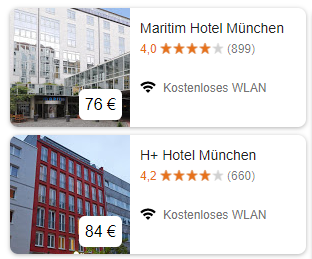
\includegraphics[width = 0.35\linewidth]{images/booking1.png} ~~~ 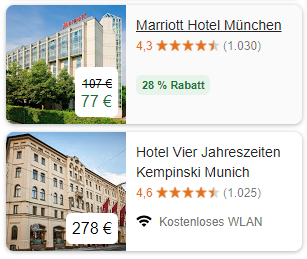
\includegraphics[width = 0.35\linewidth]{images/booking2.png}
\end{center}

When booking a hotel: find the hotel with

\begin{itemize}
\item Minimum price per night (\textbf{costs}) and
\item Maximum user rating (\textbf{performance}).
\end{itemize}

\vfill

\begin{footnotesize}
Since we limit ourselves to minimizing problems, we minimize negative valuations.
\end{footnotesize}

\framebreak

The goals often conflict with each other:

\begin{itemize}
\item Lower price $\to$ often lower hotel rating.
\item Better rating $\to$ usually higher price.
\end{itemize}

Example: (negative) average rating by hotel guests (1 - 5) vs. average price per night in USD from hotels on Expedia (excerpt).

\vspace*{0.2cm}

\centering 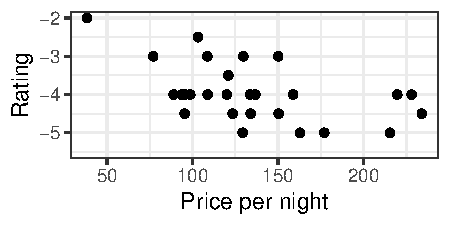
\includegraphics[scale=1]{images/expedia-1-1}


\framebreak

In addition, targets are often not comparable because they have different units, for example:

\begin{itemize}
    \item Left: a hotel with rating $4$ for $89$ Euro ($\textcolor{green}{\cost^{(1)}} = \left(89, - 4.0\right)$ would be preferred to a hotel $\textcolor{red}{\cost^{(2)}} = \left(108, - 4.0\right)$)
\item Right: how to decide if $\textcolor{orange}{\cost^{(1)}} = \left(89, - 4.0\right)$ and $\textcolor{orange}{\cost^{(1)}} = \left(95, - 4.5\right)$?
\item How much money is one \textit{rating point} worth?
\end{itemize}

\centering 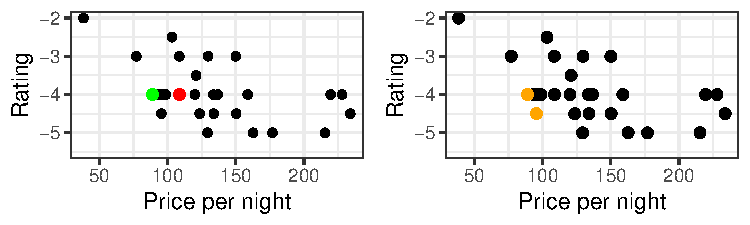
\includegraphics[scale=1]{images/expedia-2-1}

\end{frame}


\begin{frame}{Definition: multi-criteria optimization problem}

Let $\pcs \subset \realnum^n$ and $\cost: \pcs \to \realnum^m$, $m \ge 2$. A \textbf{multi-criteria optimization problem} is defined by

$$
\min_{\conf \in \pcs}  \cost(\conf) \Leftrightarrow \min_{\conf \in \pcs} \left(\cost_1(\conf), \cost_2(\conf), ..., \cost_m(\conf)\right).
$$

\begin{itemize}
\item \textbf{Goal:} minimize multiple target functions simultaneously.
\item Objective functions are often conflicting.
\item Often no clear best solution, but a set of solutions that are equally good.
\item Synonym terms: multi-criteria optimization, multi-objective optimization, Pareto optimization
\end{itemize}

\end{frame}

\begin{frame}{Pareto sets und Pareto optimality}

\textbf{Definition:}

Given a multicriteria optimization problem
    $$\min_{\conf \in \pcs} \cost(\conf) = \left(\cost_1(\conf), ..., \cost_m(\conf)\right), \quad \cost_i: \pcs \to \realnum.$$

\begin{itemize}
    \item A solution $\conf^{(1)}$ \textbf{(Pareto-) dominates} $\conf^{(2)}$, if $\cost(\conf^{(1)}) \prec \cost(\conf^{(2)})$, i.e.
\begin{enumerate}
    \item $\cost_i(\conf^{(1)}) \le \cost_i(\conf^{(2)})$ for all $i \in \{1, 2, ..., m\}$ and
    \item $\cost_j(\conf^{(1)}) < \cost_j(\conf^{(2)})$ for at least one $j \in \{1, 2, ..., m\}$
\end{enumerate}
\vspace*{0.1cm}
\item A solution $\optconf$ that is not dominated by any other solution is called \textbf{Pareto optimal}.
\vspace*{0.1cm}
\item The set of all Pareto optimal solutions is called \textbf{Pareto set} $\mathcal{P} := \{\conf \in \pcs |\not \exists ~\tilde{\conf} \text{ with } \cost(\tilde{\conf}) \prec \cost(\conf)\}$
\item $\mathcal{F} = \cost(\mathcal{P}) = \{\cost(\conf) | \conf \in \mathcal{P}\}$ is called \textbf{Pareto front}.
\end{itemize}

\end{frame}


\begin{frame}[allowframebreaks]{How to define optimality?}

Let still $\cost = (\text{price}, - \text{rating})$. For some cases it is \textit{clear} which point is the better one:

\begin{itemize}
    \item The solution $\textcolor{green}{\cost^{(1)}} = \left(89, - 4.0\right)$ dominates $\textcolor{red}{\cost^{(2)}} = \left(108, - 4.0\right)$: $\textcolor{green}{\cost^{(1)}}$ is not worse in any dimension and is better in one dimension. $\textcolor{red}{\cost^{(2)}}$ gets \textbf{dominated} by $\textcolor{green}{\cost^{(1)}}$
$$
\textcolor{red}{\cost^{(2)}} \prec \textcolor{green}{\cost^{(1)}}.
$$
\end{itemize}

\centering 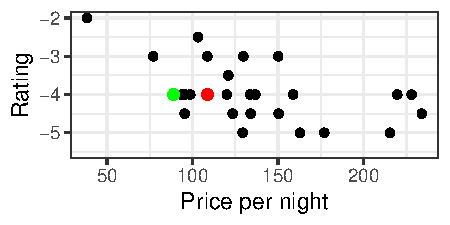
\includegraphics[width=0.5\linewidth]{images/expedia-3-1}

\framebreak

For the points $\textcolor{orange}{\cost^{(1)}} = \left(89, - 4.0\right)$ and $\textcolor{orange}{\cost^{(2)}} = \left(95, - 4.5\right)$ we cannot say which one is better.

\begin{itemize}
\item We define the points as \textbf{equivalent} and write

$$
\textcolor{orange}{\cost^{(1)}} \not\prec \textcolor{orange}{\cost^{(2)}} \text{ and } \textcolor{orange}{\cost^{(2)}} \not\prec \textcolor{orange}{\cost^{(1)}}.
$$

\centering 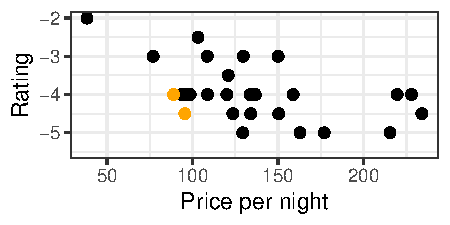
\includegraphics[width=0.5\linewidth]{images/expedia-4-1}


\item The set of all equivalent points that are not dominated by another point is called the \textbf{Pareto front}.

\vspace*{0.3cm}

\centering 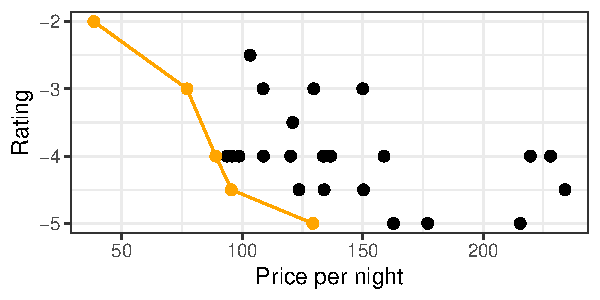
\includegraphics[width=0.8\linewidth]{images/expedia-5-1}



\end{itemize}

\end{frame}

\begin{frame}{Example: An Objective Function}


We consider the minimization problem

$$
\min_{\conf} \cost(\conf) = (\conf - 1)^2, \qquad 0 \le \conf \le 3.
$$

The optimum is at $\optconf = 1$.

\vspace*{0.1cm}


\centering 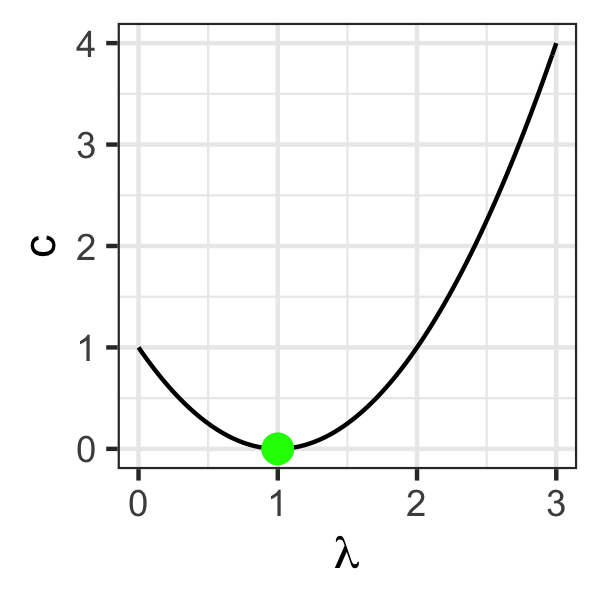
\includegraphics[scale=0.2]{images/graph1}


\end{frame}

\begin{frame}[allowframebreaks]{Example: two target functions}

We extend the above problem to two objective functions $\cost_1(\conf) = (\conf - 1)^2$ and $\cost_2(\conf) = 3(\conf - 2)^2$, thus

$$
    \min_{\conf} \cost(\conf) := \left(\cost_1(\conf), \cost_2(\conf)\right), \qquad 0 \le \conf \le 3.
$$

    \begin{center}
    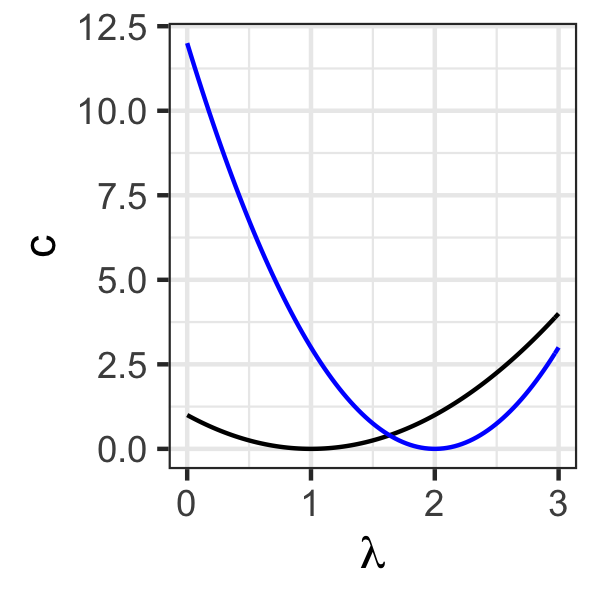
\includegraphics[scale=0.2]{images/graph2}
    \end{center}

\framebreak

We consider the functions in the objective function space $\cost(\pcs)$ by drawing the objective function values $\left(\cost_1(\conf), \cost_2(\conf)\right)$ for all $0 \le \conf \le 3$.

\vspace*{0.1cm}


    \begin{center}
    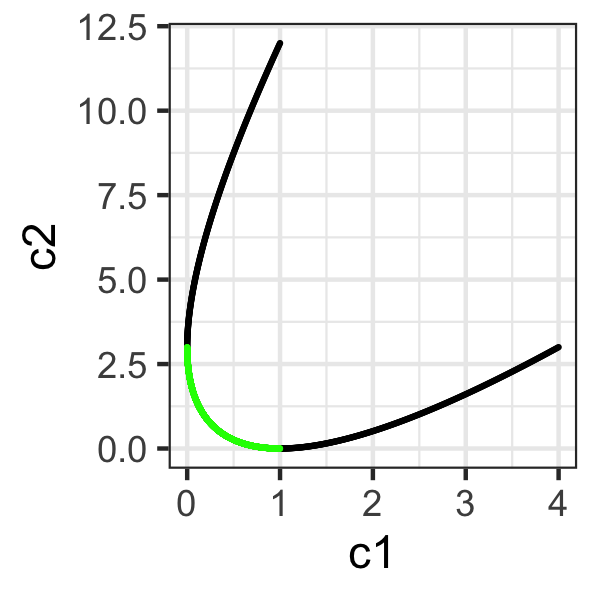
\includegraphics[scale=0.2]{images/graph3}
    \end{center}
    \vspace*{-0.3cm}

The Pareto front is shown in green.
The Pareto front cannot be \enquote{left} without getting worse in at least one objective function.

\end{frame}


\begin{frame}{Two solutions}

\begin{itemize}
\item The Pareto set is a set of equally optimal solutions.
\item In many applications one is often interested in a \textbf{single} optimal solution.
\item Without further information no unambiguous optimal solution can be determined \\
$\to$ decision must be based on other criteria.
\end{itemize}

There are two possible approaches:
\begin{itemize}
\item \textbf{A-priori approach}: user preferences are considered \textbf{before} the optimization process
\item \textbf{A-posteriori approach}: user preferences are considered \textbf{after} the optimization process
\end{itemize}

\end{frame}

\begin{frame}[allowframebreaks]{A-priori procedure}

\textbf{Example: weighted total}


\textbf{Prior knowledge:} one rating point is worth $50$ Euro to a customer. \\ $\to$ We optimize the weighted sum:

$$
\min_\text{Hotel} \text{(Price / Night)} - 50 \cdot \text{Rating}
$$

    \begin{center}
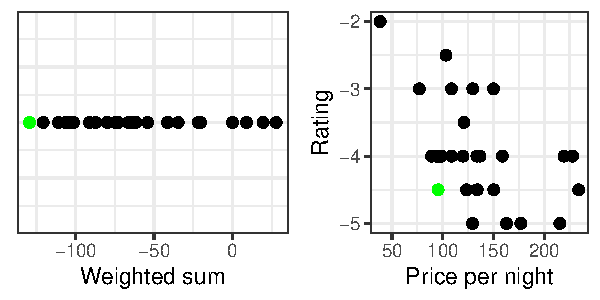
\includegraphics[scale=0.555555]{images/expedia-9-1}
    \end{center}

    Alternative weighted sum: $\min_{\conf \in \pcs} \sum_{i = 1}^m w_i \cost_i(\conf) \qquad \text{with} \quad w_i \ge 0 $
% Bei systematischem Variieren der Gewichte können alle Lösungen auf dem konvexen Zielbereich gefunden werden.

\framebreak

\textbf{Example: Lexicographic method}

\lz

\textbf{Prior knowledge:} customer prioritizes rating over price. \\
$\to$ optimize target functions one after the other.

\lz

    \begin{center}
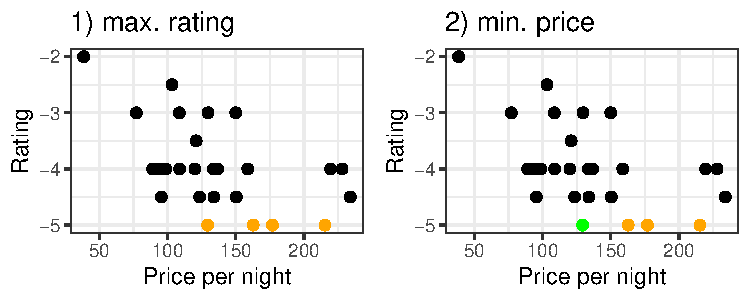
\includegraphics[scale=1]{images/expedia-10-1}
    \end{center}

\framebreak

A-priori approach: Lexicographic method

\begin{eqnarray*}
y_1^* &=& \min_{\conf \in \pcs} \cost_1(\conf)\\
y_2^* &=& \min_{\conf \in \{\conf ~|~ \cost_1(\conf) = y_1^*\}} \cost_2(\conf) \\
y_3^* &=& \min_{\conf \in \{\conf ~|~ \cost_1(\conf) = y_1^* \land \cost_2(\conf) = y_2^*\}} \cost_3(\conf) \\
&\vdots&
\end{eqnarray*}

But: different sequences provide different solutions.

\framebreak

\textbf{Summary a-priori approach:}
\begin{itemize}
\item In a single application, only one solution is obtained, which depends on the a-priori selection of weights, order, etc.
\item In case of repeated use, several solutions are obtained if weights, order, etc. are systematically varied.
\item Usually there are solutions that remain hidden from these methods.
\item Implicit assumption: single-criteria optimization is \enquote{simple}.
\end{itemize}

\end{frame}

\begin{frame}[allowframebreaks]{A-posteriori procedure}

A-posteriori methods, on the other hand, have the goal to

\begin{itemize}
\item find the set of \textbf{all} optimal solutions (the Pareto set),
\item select (if necessary) an optimal solution based on prior knowledge or individual preferences.
\end{itemize}

A-posteriori methods are therefore the more generic approach to solving a multi-criteria optimization problem.


\framebreak

\textbf{Example:} A user gets more detailed information about all Pareto optimal hotels (left) and chooses an optimal solution (right) based on previous knowledge or additional criteria (e.g. location of the hotel).

\vspace*{0.1cm}


\centering 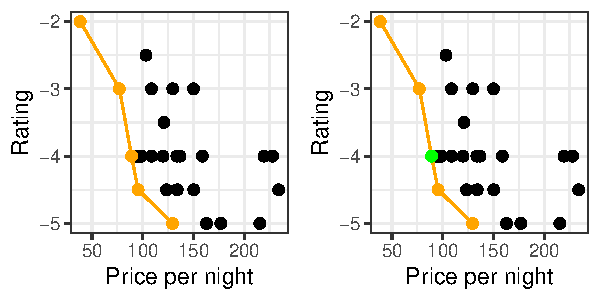
\includegraphics[scale=1]{images/expedia-11-1}


\end{frame}


\begin{frame}[allowframebreaks]{Evaluation of solutions}

A common metric for evaluating the performance of a set of solutions $\mathcal{P} \subset \pcs$ is the \textbf{dominated hypervolume}

$$
    S(\mathcal{P}, R) = \Lambda\left(\bigcup_{\tilde{\conf} in \mathcal{P}}\left\{\conf | \tilde{\conf} \prec \conf \prec R\right\}\right),
$$

where $\Lambda$ is the Lebuesge measure.
    \vspace{1cm}
    \begin{itemize}
            \item The dominated hypervolume is calculated respective to the reference point $R$, that can be chosen arbitrarely.
            \item Exact computation of the hypervolume is expensive (NP-hard), but fast approximations exist.
            \item The dominated hypervolume is also often called \textbf{S-Metric}.
    \end{itemize}

\framebreak

\begin{center}
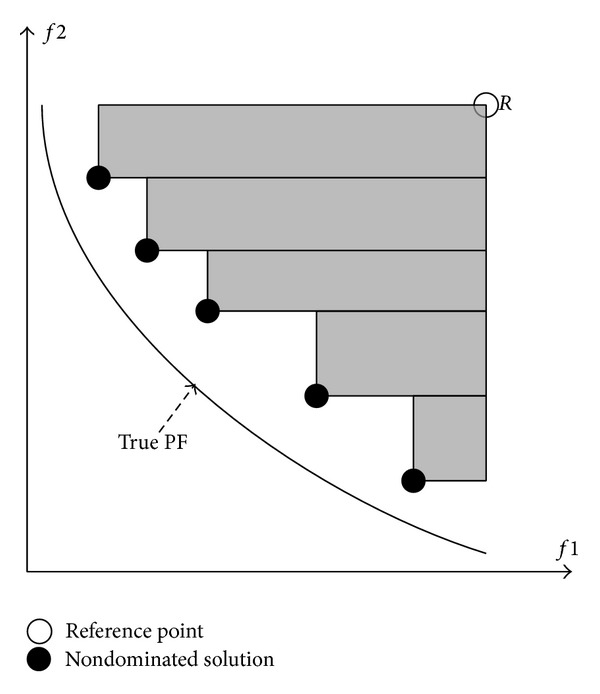
\includegraphics[width = 0.3\linewidth]{images/dominated_hypervolume.png}
\end{center}

The dominated hypervolume of $\mathcal{P}$ (5 black points) is the area in the target function space (in respect to the reference point $R$) which is dominated by points $\mathcal{P}$.

\framebreak



\end{frame}

\end{document}
